
\documentclass[a4paper,11pt]{report}
\usepackage[utf8]{inputenc}
\usepackage[T1]{fontenc}
\usepackage{lmodern}
\usepackage[ngerman]{babel}
\usepackage[margin=20mm, left=20mm, right=10mm, headheight=15pt, includeheadfoot]{geometry}
\usepackage{fancyhdr}
\usepackage{opensans}
\usepackage{titlesec}
\usepackage{tocloft}
\usepackage{titling}
\usepackage{hyperref}
\usepackage{graphicx}
\usepackage{enumerate}
\usepackage{float}
\usepackage{caption}
\usepackage{listings}
\usepackage{wrapfig}
\usepackage{minted}
\usemintedstyle{vs}

% Set default font to OpenSans
\renewcommand*\familydefault{\sfdefault}

% Page style for cover page
\fancypagestyle{cover}{
    \fancyhf{}
    \renewcommand{\headrulewidth}{0pt}
    \renewcommand{\footrulewidth}{0pt}
}

% Page style for main content
\fancypagestyle{main}{
    \fancyhf{}
    \fancyhead[L]{\theauthor}
    \fancyhead[R]{\subject}
    \fancyfoot[C]{\thepage}
    \renewcommand{\headrulewidth}{0.4pt}
    \renewcommand{\footrulewidth}{0pt}
}

\titleformat{\chapter}[block]
  {\normalfont\Large\bfseries} % change \Large to \large or any other size that fits
  {\thechapter}
  {1em}
  {}

  \titlespacing*{\chapter}{0pt}{*4}{*2.5}

% Cover page
\newcommand{\coverpage}{
    \thispagestyle{cover}
    \pagenumbering{roman} % Start Roman numbering for the cover page
    \begin{center}
        {
\includegraphics[height=3cm]{fh-logo}}\\[1cm]
        {\LARGE \thetitle}\\[0.5cm]
        {\large \theauthor}\\
    \end{center}
    \tableofcontents
    \clearpage
}

% Author and subject
\author{Felix Hillebrand}
\newcommand{\subject}{AMS4UE}

\graphicspath{ {./images/}{./notebooks/images} }

% Main document
\begin{document}
    % Color definitions
    \definecolor{LightGray}{gray}{0.9}
    \definecolor{DarkGray}{gray}{0.3}

    \title{AMS~-~UE}
    \coverpage

    \clearpage
    \pagestyle{main}
    \pagenumbering{arabic} % Start Arabic numbering for main content

% ------------------------------------------
% --        Main document starting        --
% ------------------------------------------

    \chapter{Spannbaum Prim}
    \label{ch:spbprim}
    Suchen Sie einen minimalen Spannbaum mit dem Algorithmus von Prim und stellen Sie diesen dar.
    Welche Kosten hat dieser?

    \begin{figure}[H]
        \centering
        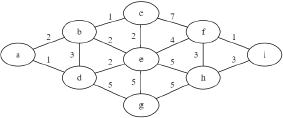
\includegraphics[width=0.6\textwidth]{a01a_graph}
        \label{fig:a01_graph}
    \end{figure}

    \newpage

    \chapter{Spannbaum Kruskal}
    \label{ch:sbkruskal}
    Für den Graphen aus \hyperref[fig:a01_graph]{Beispiel~1} suchen Sie einen minimalen Spannbaum mit dem Algorithmus von
    Kruskal und stellen Sie diesen dar. Unterscheidet sich dieser vom Spannbaum in Beispiel 1?

    \newpage

    \chapter{Minimale Spannbäume}
    \label{ch:minSb}
    \begin{enumerate}
        \item Suchen Sie alle minimalen Spannbäume (MST) in folgendem Graph.
        Welche Kosten weisen diese auf?
        Stellen Sie die unterschiedlichen MST dar!

        \begin{figure}[H]
            \centering
            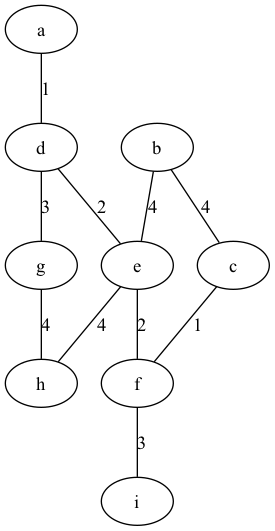
\includegraphics[width=0.6\textwidth]{a03a_graph}
            \label{fig:a03_graph}
        \end{figure}
        \item
        \item Gegeben ein minimaler Spannbaum T von einem Graph $G$.
        Wie kann geprüft werden ob es weitere MST in $G$ gibt oder ob $T$ einzigartig ist?
    \end{enumerate}

    \newpage

    \chapter{Die MST-Heuristik für das TSP}
    \label{ch:mstHeuristicTSP}
    Eine bewährte Methode gute (wenn auch nicht optimale) Rundreisen zu finden, fußt auf minimalen Spannbäumen.
    Bilden Sie für den Graphen $G$ (siehe Code unten), eine solche heuristische Rundreise mittels MST-Heuristik.
    Ermitteln Sie dazu:

    \begin{enumerate}[a)]
        \item einen minimalen Spannbaum MST
        \item einen gerichteten Graphen $G2$ bei dem jede Verbindung in MST durch eine Hin- und
        eine Zurückkante dargestellt wird
        \item einen Eulerkreis $k$ in $G2$ der in Linz beginnt und endet
        \item einen Hamiltonkreis $r$ in $G$ in dem Sie $k$ folgen und bereits besuchte Knoten
        überspringen
    \end{enumerate}

    \begin{minted}[
        frame=lines,
        framesep=2mm,
        baselinestretch=1.2,
        bgcolor=LightGray,
        linenos,
        breaklines
    ]{python}
G = nx.Graph()
G.add_weighted_edges_from([
    ("Wien", "Linz",184.4),
    ("Wien", "Hagenberg",180),
    ("Wien", "Graz",200.1),
    ("Wien", "Salzburg",295),
    ("Wien", "Steyr",166),
    ("Wien", "Wels",197),
    ("Linz", "Hagenberg",23),
    ("Linz", "Graz",220.9),
    ("Linz", "Salzburg",132.5),
    ("Linz", "Wels",132.5),
    ("Linz", "Steyr",132.5),
    ("Salzburg", "Steyr",134),
    ("Salzburg", "Graz",296),
    ("Salzburg", "Wels",108),
    ("Salzburg", "Hagenberg",155),
    ("Graz", "Steyr",191),
    ("Graz", "Wels",196),
    ("Graz", "Hagenberg",243),
    ("Wels", "Steyr",45.2),
    ("Wels", "Hagenberg",57.2),
    ("Steyr", "Hagenberg",43.6)
])
    \end{minted}

    \newpage

    \chapter{Minimale Spannbäume in gerichteten Graphen}
    \label{ch:minSbDiGraph}
    Recherchieren Sie nach minimalen Spannbäumen für gerichtete Graphen.
    Sind die Algorithmen von Prim und Kruskal für gerichtete Graphen anwendbar?
    Warum (nicht)?

    \newpage

    \chapter{PageRank}
    \label{ch:pageRank}
    Bestimmen Sie die Matrizen $\widetilde{A}$, $\widetilde{A}$ und $M$ für den Dämpfungsfaktor $d = 0.75$ und stellen Sie diese dar.
    Berechnen Sie den PageRank, geben Sie den Vektor $R$ nach den ersten $3$ Iterationen aus dem Potenzverfahren an (Initialwert $R_0$, $R_1$, $R_2$, $R_3$) wobei die Zahl im Index für die Iteration steht.
    Was bedeutet der PageRank?

    \begin{figure}[H]
        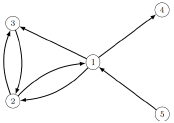
\includegraphics[width=0.3\textwidth]{a06a_graph}
        \label{fig:a06_graph}
    \end{figure}

    \newpage

    \chapter[Page Rank als Simulation]{Page~Rank als Simulation}
    \label{ch:pageRankSim}

    \begin{wrapfigure}{r}{0.32\textwidth}
        \centering
        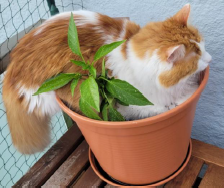
\includegraphics[width=0.3\textwidth]{a07a_cat}
        \label{fig:a06_cat}
    \end{wrapfigure}

    Aurora hat in der Küche zu viel Katzengras erwischt und ist dementsprechend berauscht.
    Sie können die Katze im untenstehenden Routinggraf der Wohnung Ihres Übungsleiters als „Random cat-agent“ annehmen,
    der in jedem Zeitschritt zufällige Kanten wählt (auch zurück).
    Wenn die Katze eines der drei Katzenbetten erreicht, legt sie sich dort schlafen (Katzenbetten sind Senken).
    In welchem Bett wird Sie die Katze mit welcher Wahrscheinlichkeit nach einer sehr großen Anzahl an Zeitschritten auffinden?
    Nach wie vielen Iterationen beträgt die Gesamtwahrscheinlichkeit, dass die Katze irgendein Bett erreicht, hat über 30\%?

    \begin{figure}[h]
        \centering
        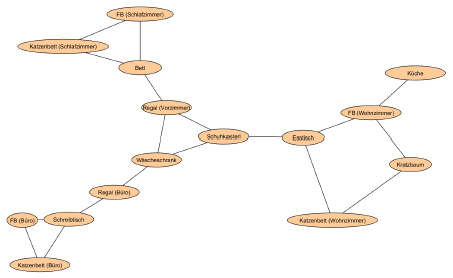
\includegraphics[width=0.8\textwidth]{a07a_graph}
        \label{fig:a07_graph}
    \end{figure}


    \newpage

    \chapter{Legal}
    \label{ch:legal}
    Die Ausarbeitung der Aufgabe wurde durch:

    \begin{itemize}
        \item \texttt{OpenAI - GPT-4.5 Turbo}
        \item \texttt{OpenAI - GPT-4.5 Vision}
        \item \texttt{OpenAI - GPT-4o}
        \item \texttt{Anthropic -- Claude 3 Opus}
    \end{itemize}

    mit mehreren unterschiedlichen Prompts und Custom Instructions unterstützt.

\end{document}